% \setcounter{chapter}{2}
\chapter{Forward Kinematics}
\section{Important}
Read the entire lab before starting and especially the ``Grading" section so you are aware of all due dates and requirements associated with the lab.  Hopefully you are reading this well before your lab section meets as given the compressed schedule, it is very important that you arrive at lab well prepared.  This semester, the more you do prior to your lab session, the more you will get out of the short time you have with the TA.
\section{Objectives}
The purpose of this lab is to implement the exponential forward kinematics on the UR3e robot to estimate the end-effector pose given a set of joint angles.  In this lab you will:
\begin{itemize}
	\item Solve the exponential forward kinematic equations for the UR3e.
	\item Write a Python function that moves the UR3e to a configuration specified by the user.
	\item Compare your exponential forward kinematic estimation with the actual robot movement. 
\end{itemize}

\section{References}
\begin{itemize}
\item Chapter 4 of \textit{Modern Robotics} provides details of how to construct an exponential forward kinematic for an open-chain robot.
\end{itemize}

\section{Tasks}

\subsection{Theoretical Solution}
Find the forward kinematic equations for the UR3e robot using the exponential forward kinematics method.  Solve for $T_{06}$ and record the 6 matrices defined by $e^{[S_1]\theta_1}$ through $e^{[S_6]\theta_6}$.

\subsection{Physical Implementation} \label{sec:physical}
The user will provide six joint angles $\left\{\theta_1,\theta_2,\theta_3,\theta_4,\theta_5,\theta_6\right\}$, all given in degrees.  The angle ranges are as follows:

\begin{eqnarray*}
-90^{\circ}<&\theta_1&<90^{\circ}\\
-180^{\circ}<&\theta_2&<0^{\circ}\\
-5^{\circ}<&\theta_3&<140^{\circ}\\
-95^{\circ}<&\theta_4&<-5^{\circ}\\
-115^{\circ}<&\theta_5&<70^{\circ}\\
-170^{\circ}<&\theta_6&<170^{\circ}
\end{eqnarray*}

Note that these ranges are approximate and vary slightly from machine to machine.  If you receive a protective stop, note the affected joint on the teach pendant and make appropriate corrections. 
It is also worth noting that not all configurations are achievable or desirable.  Some will strike the table or wall or be difficult to measure accurately. 
These limits are primarily for the real robot and will not affect the simulation, but it is advised that you make use of them to achieve realistic configurations.

Once the angles are selected, using the ROS Python program move the joints to these desired angles.  Your program should additionally calculate and display the translation\
matrix $T_{06}$ that rotates and translates the end effector's coordinate frame to the base frame.

\subsection{Comparison}
For any provided set of joint angles $\left\{\theta_1,\theta_2,\theta_3,\theta_4,\theta_5,\theta_6\right\}$, compare the measured position or the position output from the ROS topic with the value calculated by your Python forward kinematics function.  

\section{Procedure}
	
\subsection{Theoretical Solution}
\begin{enumerate}
\item In exponential forward kinematics (especially for an open chain kinematics), there are three components that are essential for the calculation.
    \begin{itemize}
    \item A fixed base frame $f_0$
    \item Robot's “zero” configuration (or some might call it initial position)
    \item A well-defined end-effector frame $f_6$
    \end{itemize}

Practically, you can define the base frame, the end-effector frame, and zero configuration arbitrarily. As long as you remain consistent with your definitions, the end results will be identical for the same robot. 
However, doing so will pose difficulties when your TA tries to verify your answer or debug your process. Therefore we encourage you to use the same frame placement and zero configuration for both convenience and safety purposes. See \figref{UR3e_zero_config}.  
For convenience when measuring, the base frame, $f_{0}$, is placed at the middle of robot's base.

\begin{figure}[h]
	\centering
		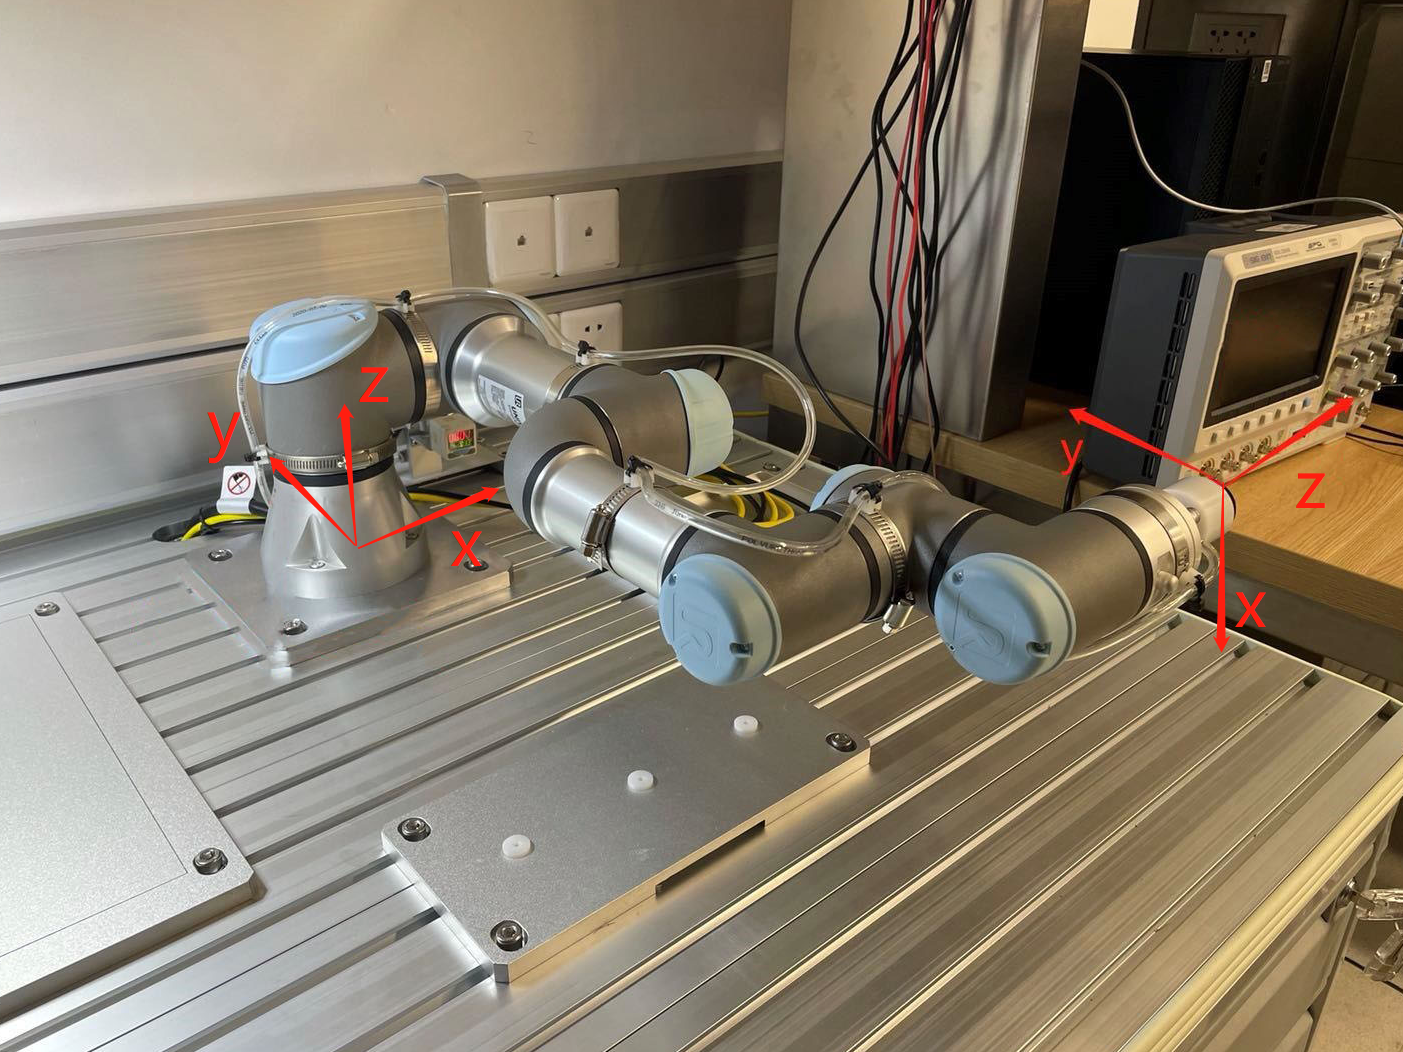
\includegraphics[height=3.4in]{image/lab4_zero_config.jpg}
	\caption{\figlbl{UR3e_zero_config} “zero” configuration and frame placement for UR3e.}
\end{figure}

Moreover, please note that in this lab, all the UR3e robots have a pre-defined zero configuration. The pose shown in \figref{UR3e_zero_config} is \textbf{NOT the TRUE zero configuration} according to the teach pendant. In this pose (\figref{UR3e_zero_config}), you would read the following joint angles from \textbf{the teach pendant}:

\begin{center}
\begin{tabular}{ |c|c|c|c|c|c| } 
\hline
Joint 1 & Joint 2 & Joint 3 & Joint 4 & Joint 5 & Joint 6\\
\hline
90.0$^{\circ}$ & 0.0$^{\circ}$ & 0.0$^{\circ}$ & -90.0$^{\circ}$ & 0.0$^{\circ}$ & 0.0$^{\circ}$\\ 
\hline
\end{tabular}
\end{center}
In the  \textbf{teach pendant's} zero configuration, (due to how the robot is originally mounted) the robot arm would face the far edge of the table and the wrist joint would point into the table, which is an awkward pose to make measurements and do experiments. Hence, we added some angle offsets in the function script such that:

\begin{lstlisting}
	return_value[0] = theta1 + (0.5*PI)
	return_value[1] = theta2
	return_value[2] = theta3
	return_value[3] = theta4 - (0.5*PI)
	return_value[4] = theta5
	return_value[5] = theta6
\end{lstlisting}

(\textbf{Attention:} Remember in the previous lab, when we enter the angle value
on control panel into python code, the value of base and elbow should be
switched.)

\textbf{Any joint angle measurements from the robot that are passed to your ROS program will be corrected to the “zero” configuration shown in \figref{UR3e_zero_config}.}
In other words, now if you set all the joint of UR3e to zero (zero configuration) in \textbf{ROS}:
\begin{center}
\begin{tabular}{ |c|c|c|c|c|c| } 
\hline
Joint 1 & Joint 2 & Joint 3 & Joint 4 & Joint 5 & Joint 6\\
\hline
0.0$^{\circ}$ & 0.0$^{\circ}$ & 0.0$^{\circ}$ & 0.0$^{\circ}$ & 0.0$^{\circ}$ & 0.0$^{\circ}$\\ 
\hline
\end{tabular}
\end{center}
You would see the UR3e poses as \figref{UR3e_zero_config} showed.

\item The sole purpose of the forward kinematics algorithm is to estimate the end-effector's pose (orientation and position) with respect to the base frame given a set of joint angles. This information can be packed and calculated in a “homogeneous transformation matrix” as taught by Lynch \& Park in \textit{Modern Robotics}:
\begin{center}
\begin{equation*}
T(\theta) = e^{[S_1]\theta_1} e^{[S_2]\theta_2}...... e^{[S_{n-1}]\theta_{n-1}} e^{[S_n]\theta_n} M
\end{equation*}
\end{center}

While our objective is to solve for the homogeneous transformation matrix $T(\theta)$ of the “motion” caused by certain joint angle configurations, there are seven matrices we need to specify:
    \begin{itemize}
    \item The screw axes $S_1$ to $S_6$ (we have six here because UR3e has six joints) expressed in the base frame, corresponding to the joint motions when the robot is at its zero configuration (see \figref{UR3e_zero_config})
    \item The end-effector pose M (a 4x4 homogeneous transformation matrix) with respect to the base frame, corresponding to the zero configuration
    \end{itemize}
A screw axis S can be represented by $S=(\omega,v)$, where the $\omega$ is the joint axis defined by the \textbf{right hand rule} (\figref{hand}). $v$ can be computed by $v= -\omega \times q$, where q is the displacement (position) of the joint center with respect to the base frame.
\begin{figure}[t]
	\centering
		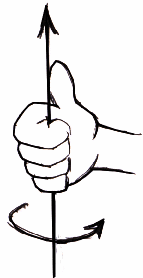
\includegraphics[scale=1]{image/lab4_hand.png}
	\caption{\figlbl{hand}The "right hand rule"}
\end{figure}

\item Using the symbolic toolbox of Matlab or Python, find the closed form solution of $T_{06}$.  You should note how long and complex the solution is due to the contribution of each joint's motion.  Additionally, calculate the 6 matrices defined by $e^{[S_1]\theta_1}$ through $e^{[S_6]\theta_6}$.

\item To aid in your calculations, several figures have been included.
\begin{itemize}
    \item \figref{UR3SA} shows the screw axes and direction of rotation (use the right rule) for each joint.
    \item \figref{UR3JC} shows the joint centers to aid in locating your $q$ values.
    \item \figref{UR3Dim} shows the dimensions of all of the links of the UR3e.
    \item \figref{EEoffset} shows the dimensions of the end effector including the aluminum plate and suction gripper.
\end{itemize}

\end{enumerate}

\subsection{Implementation on UR3e}
\begin{enumerate}
\item Copy \textbf{lab4pkg\_fk} into ``\textbf{src}" directory of your catkin directory.  Don't forget ``\textbf{source devel/setup.bash}" when you open a new terminal.  Then from your base catkin\
directory run ``\textbf{catkin\_make}" and if you receive no errors you copied your lab3 starter code correctly.  Also so that ROS registers this new package ``\textbf{lab4pkg\_fk}",
run ``\textbf{rospack list}" and you should see \textbf{lab4pkg\_fk} as one of the many packages.
\item You will notice that in \textbf{lab4pkg\_fk/scripts} there are now three *.py files.  \textbf{lab4\_exec.py} is the main() code, \textbf{lab4\_func.py} defines the important
forward kinematic functions. \textbf{lab4\_header.py} defines the header files.  We divide them up in this fashion for clarity.  In this lab you will be mainly editing
\textbf{lab4\_func.py}.  You can of course change \textbf{lab4\_exec.py} but most of its functionality has already been given to you.  Study the code and comments in
\textbf{lab4\_exec.py} and \textbf{lab4\_func.py} to see what the starter code is doing and what parts you are going to need to change. Your job is to add the code in the function \textbf{Get\_MS()} that correctly populates the six screw axes $S_1$ to $S_6$ as well as the transformation matrix M.  The Python code uses the ``numpy" module to create and multiply matrixes; meanwhile, the matrix exponential ``expm()" is achieved by including the ``Scipy" module.  Then, with the S and M values you populated, write the code in function \textbf{lab\_fk()} that generates and prints the homogeneous transformation matrix $T(\theta)$.

\item Once your code is finished, run it using ``\textbf{rosrun lab4pkg\_fk lab4\_exec.py [theta1] [theta2] [theta3] [theta4] [theta5] [theta6]}" with all angles in
degrees - e.g. \textbf{rosrun lab4pkg\_py lab4\_exec.py 0 90 45 0 -90 105}.  Remember that in another command prompt you should have first run roscore and drivers using
``\textbf{roslaunch ur\_robot\_driver ur3e\_bringup.launch}".

\item For in-person students, you should measure the x,y,z position of the end-effector using the provided ruler and square.  For students using the simulation, it is not possible to measure this way, so we must use another method.  A simple way is to use some of the ROS commands we learned before: ``\textbf{rostopic echo /gripper/position -n 1}".  These values are being calculated differently and so there will be small differences between this value and your calculations.
\item You should verify that your code works by selecting a variety of poses that will test the full range of motion.  Your TA will not be providing you test angles, so you should make use of the joint limits provided in Section \ref{sec:physical}.

\end{enumerate}
\subsection{Comparison}
\begin{enumerate}
\item Your TA will select two sets of joint angles $\left\{\theta_1,\theta_2,\theta_3,\theta_4,\theta_5,\theta_6\right\}$ when you demonstrate\
your working ROS program.  
\item Run your ROS node and move the UR3e to each of these configurations.  With a ruler and square (or the appropriate ROS command for the simulation),  measure the x,y,z position vector of the center of the gripper for each set of angles.  Call these vectors $r_1$ and $r_2$ for the first and second sets of joint angles, respectively.

\item Compare these measurements to the translation vector calculated by your ROS node.  
Call these calculated vectors $d_1$ and $d_2$.	

\item For each set of joint angles, Calculate the error between the measured and calculated kinematic solutions.  We will consider the error to be the magnitude of the distance between the measured center of the gripper and the location predicted by the forward kinematic equation:
\[
error_1 = \left\| r_1 - d_1 \right\| = \sqrt{(r_{1x}-d_{1x})^2 + (r_{1y}-d_{1y})^2 + (r_{1z}-d_{1z})^2}.
\]
A similar expression holds for $error_2$.
\end{enumerate}


\section{Report}
Each student will submit a lab report using the guidelines given in the “ECE 470: How to Write a Lab Report” document.  Please be aware of the following:
\begin{itemize}
    \item Lab reports will be submitted online at \href{https://learn.intl.zju.edu.cn/}{Blackboard}.
    \item The report will be due \textbf{2} weeks after your lab session for Lab 3.  Exact times and dates can be seen on \href{https://learn.intl.zju.edu.cn/}{Blackboard}.
\end{itemize}


Your lab report should include the following:
\begin{itemize}
\item Explain how you determined $\mathcal{S}_{1}$ thru $\mathcal{S}_{6}$ and $\textbf{M}$ - include figures as needed.
\item Include a figure that shows all frames and axes used.
\item Include a table of all $\omega$ and $q$ used and the $v$ derived.
\item Figures should be your own creation and not copies of the lab manual.

 \item Use Matlab or Python's symbolic toolbox to generate the final homogeneous transform $T_{06}$ as a function of $\left(\theta_{1},\theta_{2},\theta_{3},\theta_{4},\theta_{5},\theta_{6}\right)$.  As this is too cumbersome to include in your report, include $e^{[S_1]\theta_1}$ through $e^{[S_6]\theta_6}$ in your report (do not use screenshots).

\item Substitute in your given joint angles into your symbolic solution to verify it.
\item For each test point, include:
    \begin{itemize}
        \item The given $\left(\theta_{1},\theta_{2},\theta_{3},\theta_{4},\theta_{5},\theta_{6}\right)$
        \item The calculated $d$ and measured $r$ vectors
        \item The scalar error
        \item The output of your symbolic solution
    \end{itemize}
    \item Include a brief discussion of sources of error.
\end{itemize}
Unless your TA gives other guidance, include the following as appendices:
\begin{itemize}
    \item Your $\textbf{lab4\_func.py}$ code (and $\textbf{lab4\_exec.py}$ if it was edited).
    \item Your Matlab or Python code used to calculate the symbolic $T_{06}$.
\end{itemize}


\section{Demonstration}
Demonstrations of your working code will either be done in-person or over Zoom.  They will be done live (i.e. no recordings) with your lab section TA.  Demos are due \textbf{2} weeks after your lab session.\\

The default method of demonstrating your work will be via the simulation.  While we want to encourage in-person students to run their code on the real robot, due to time limitations, this may be difficult to do with your TA by the due date.  You can always run it for your own satisfaction at another time.
\subsection{Demo Process}
Your TA will require you to run your program twice, each time with a different set of joint variables.


\section{Grading}
\begin{itemize}
\item 80 points, successful demonstration.
\item 20 points, individual report.  
\end{itemize}


% \section{Tentative Due Dates - Fall 2020}
% The exact date and time will depend on your lab section and can be found on \href{www.gradescope.com}{GradeScope}.
% \subsection{Group A}
% \begin{itemize}
%     \item Demonstration - Week of October 19
%     \item Report - Week of October 26
% \end{itemize}

% \subsection{Group B}
% \begin{itemize}
%     \item Demonstration - Week of October 26
%     \item Report - Week of November 2
% \end{itemize}

\section{Preparation for Lab 5}
Lab 5 will cover inverse kinematics.  In class you will mostly focus on numerical inverse kinematics, but we will be using analytical inverse kinematics - i.e. we will use geometry and constraints to find a closed form solution to the problem.\\
Suggested Reading:
\begin{itemize}
    \item Chapter 6 of \textit{Modern Robotics} provides multiple examples of inverse kinematics solutions. Especially Section 6.1.
    \item Chapter 3 of \textit{Robot Modeling and Control}, by M. Spong, S. Hutchinson and M Vidyasagar (Wiley and Sons, 2005).  Especially Section 3.3.3.  (A version of this text is available online.)
\end{itemize}


\begin{figure}[t]
	\centering
		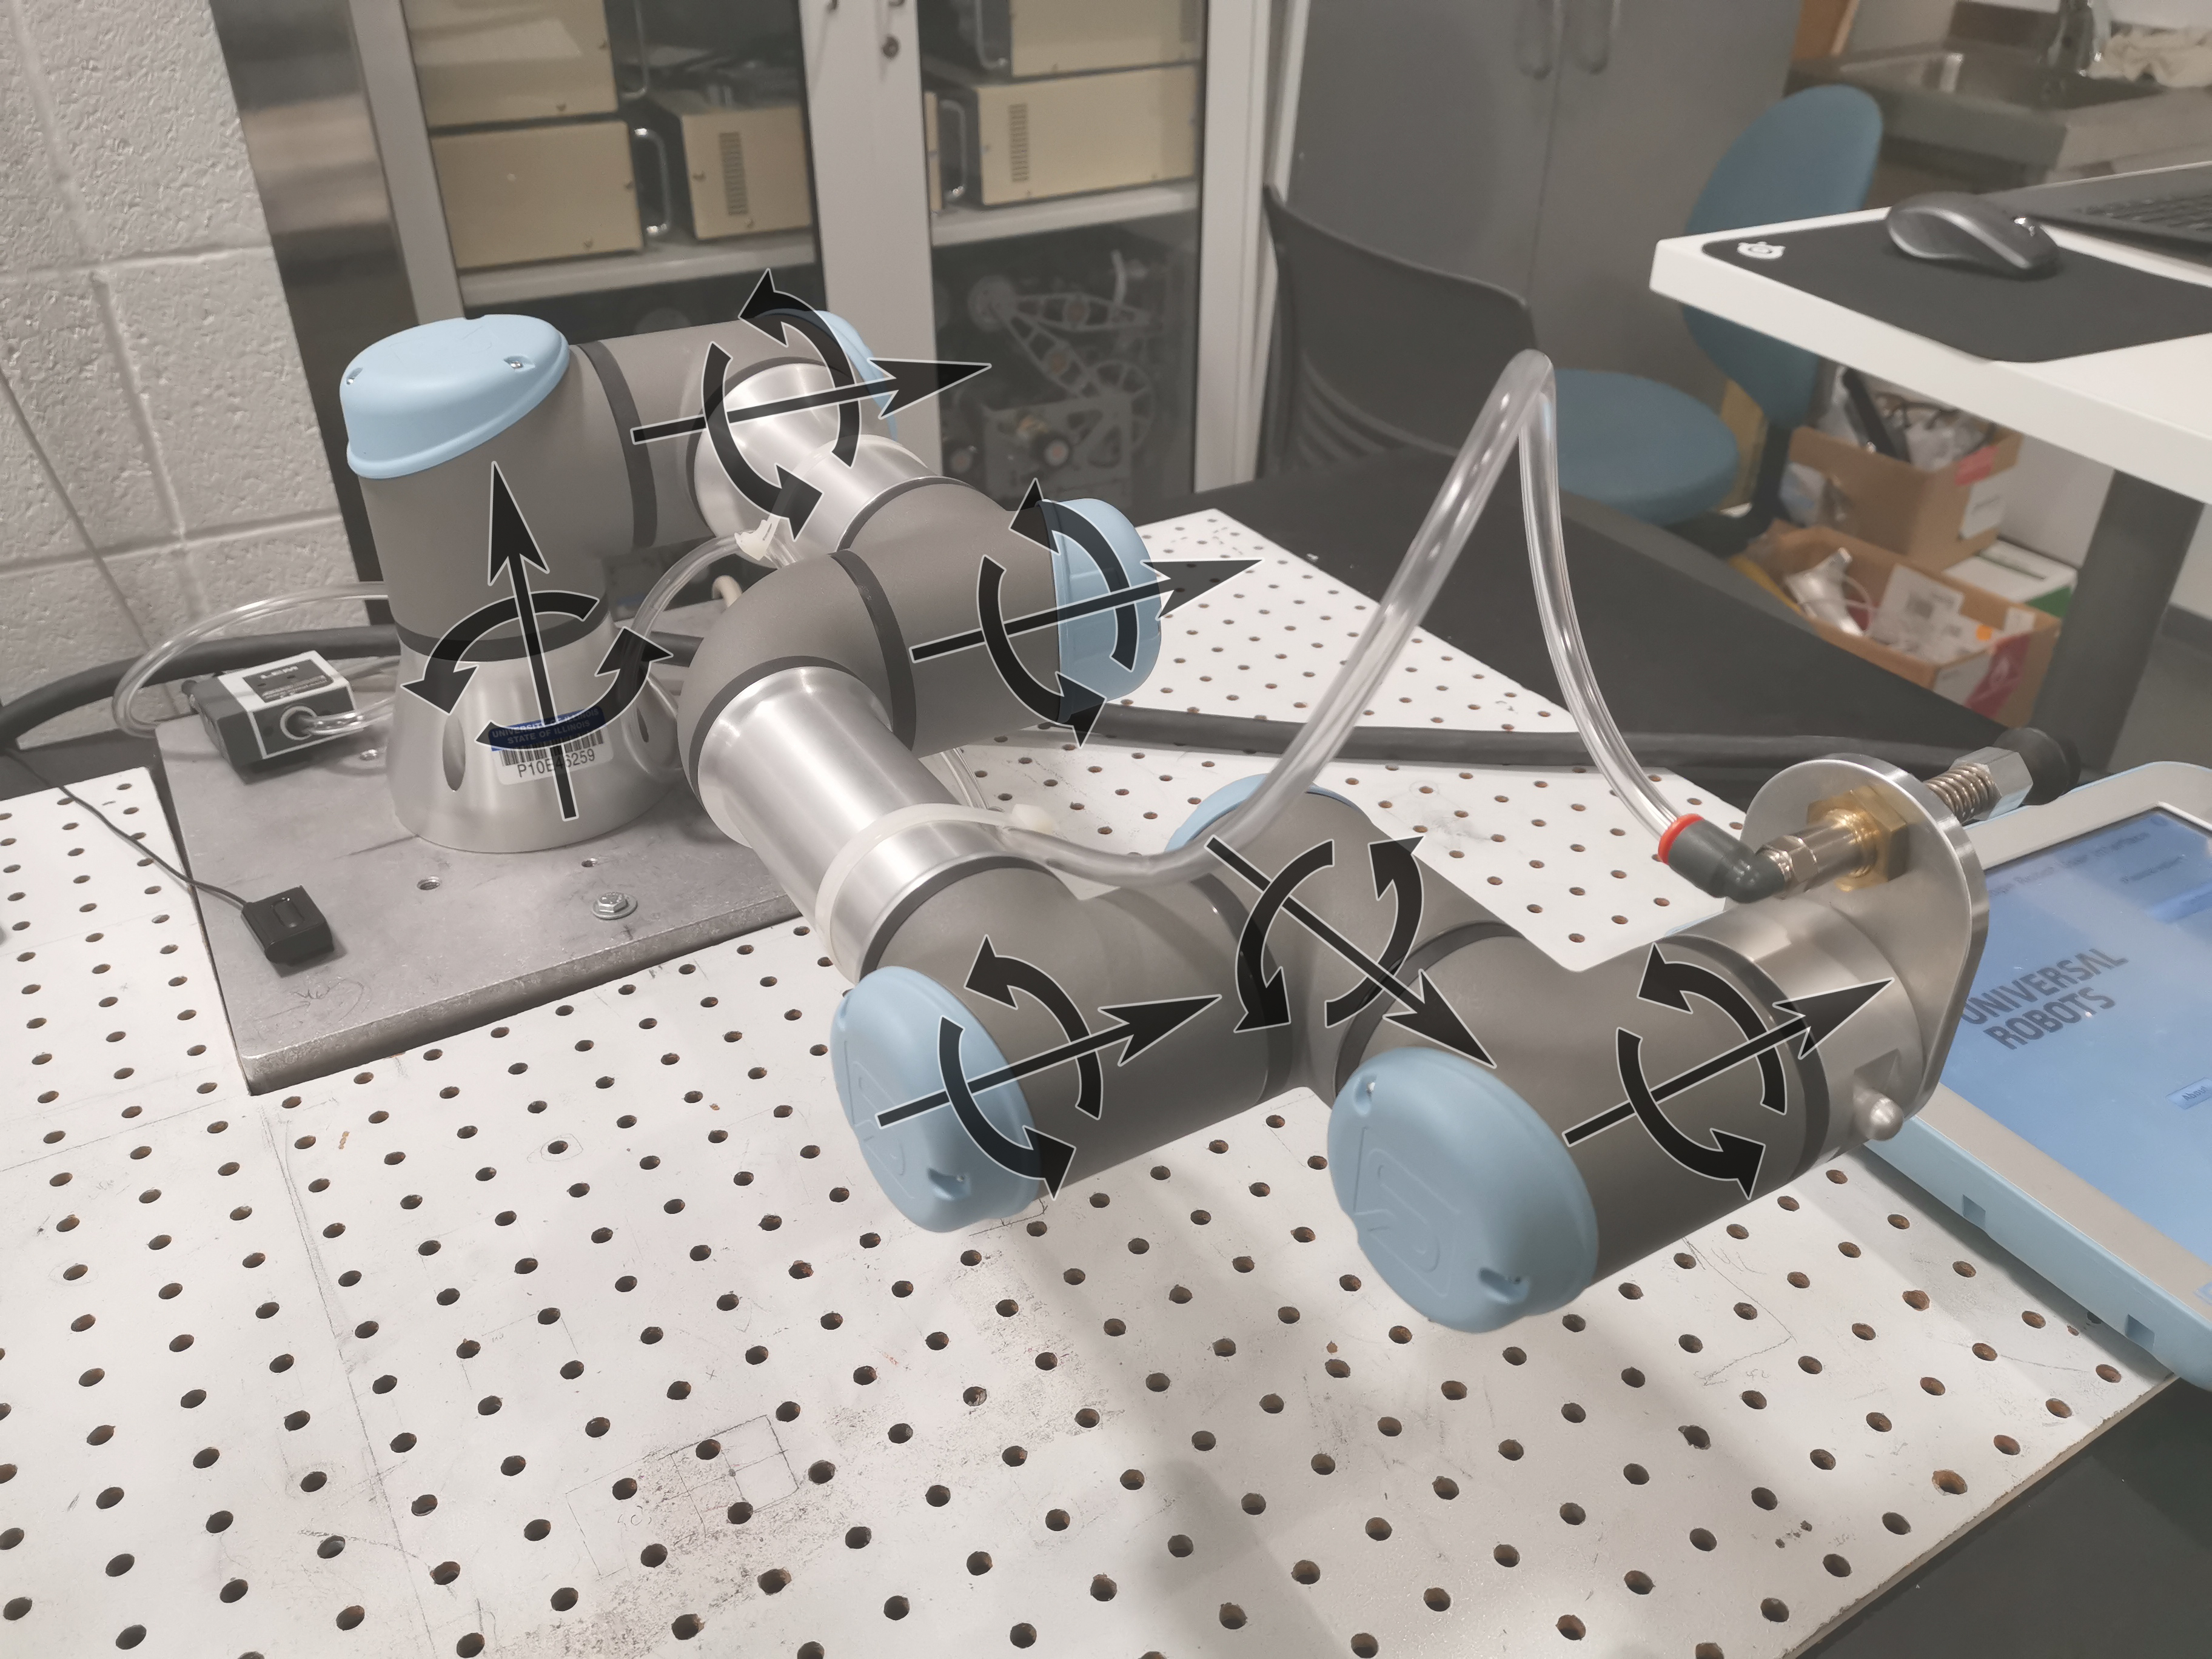
\includegraphics[height=3.4in]{image/lab4_ur3_forwardkin1.jpg}
	\caption{\figlbl{UR3SA} Screw axes on UR3e.}
\end{figure}

\begin{figure}[t]
	\centering
		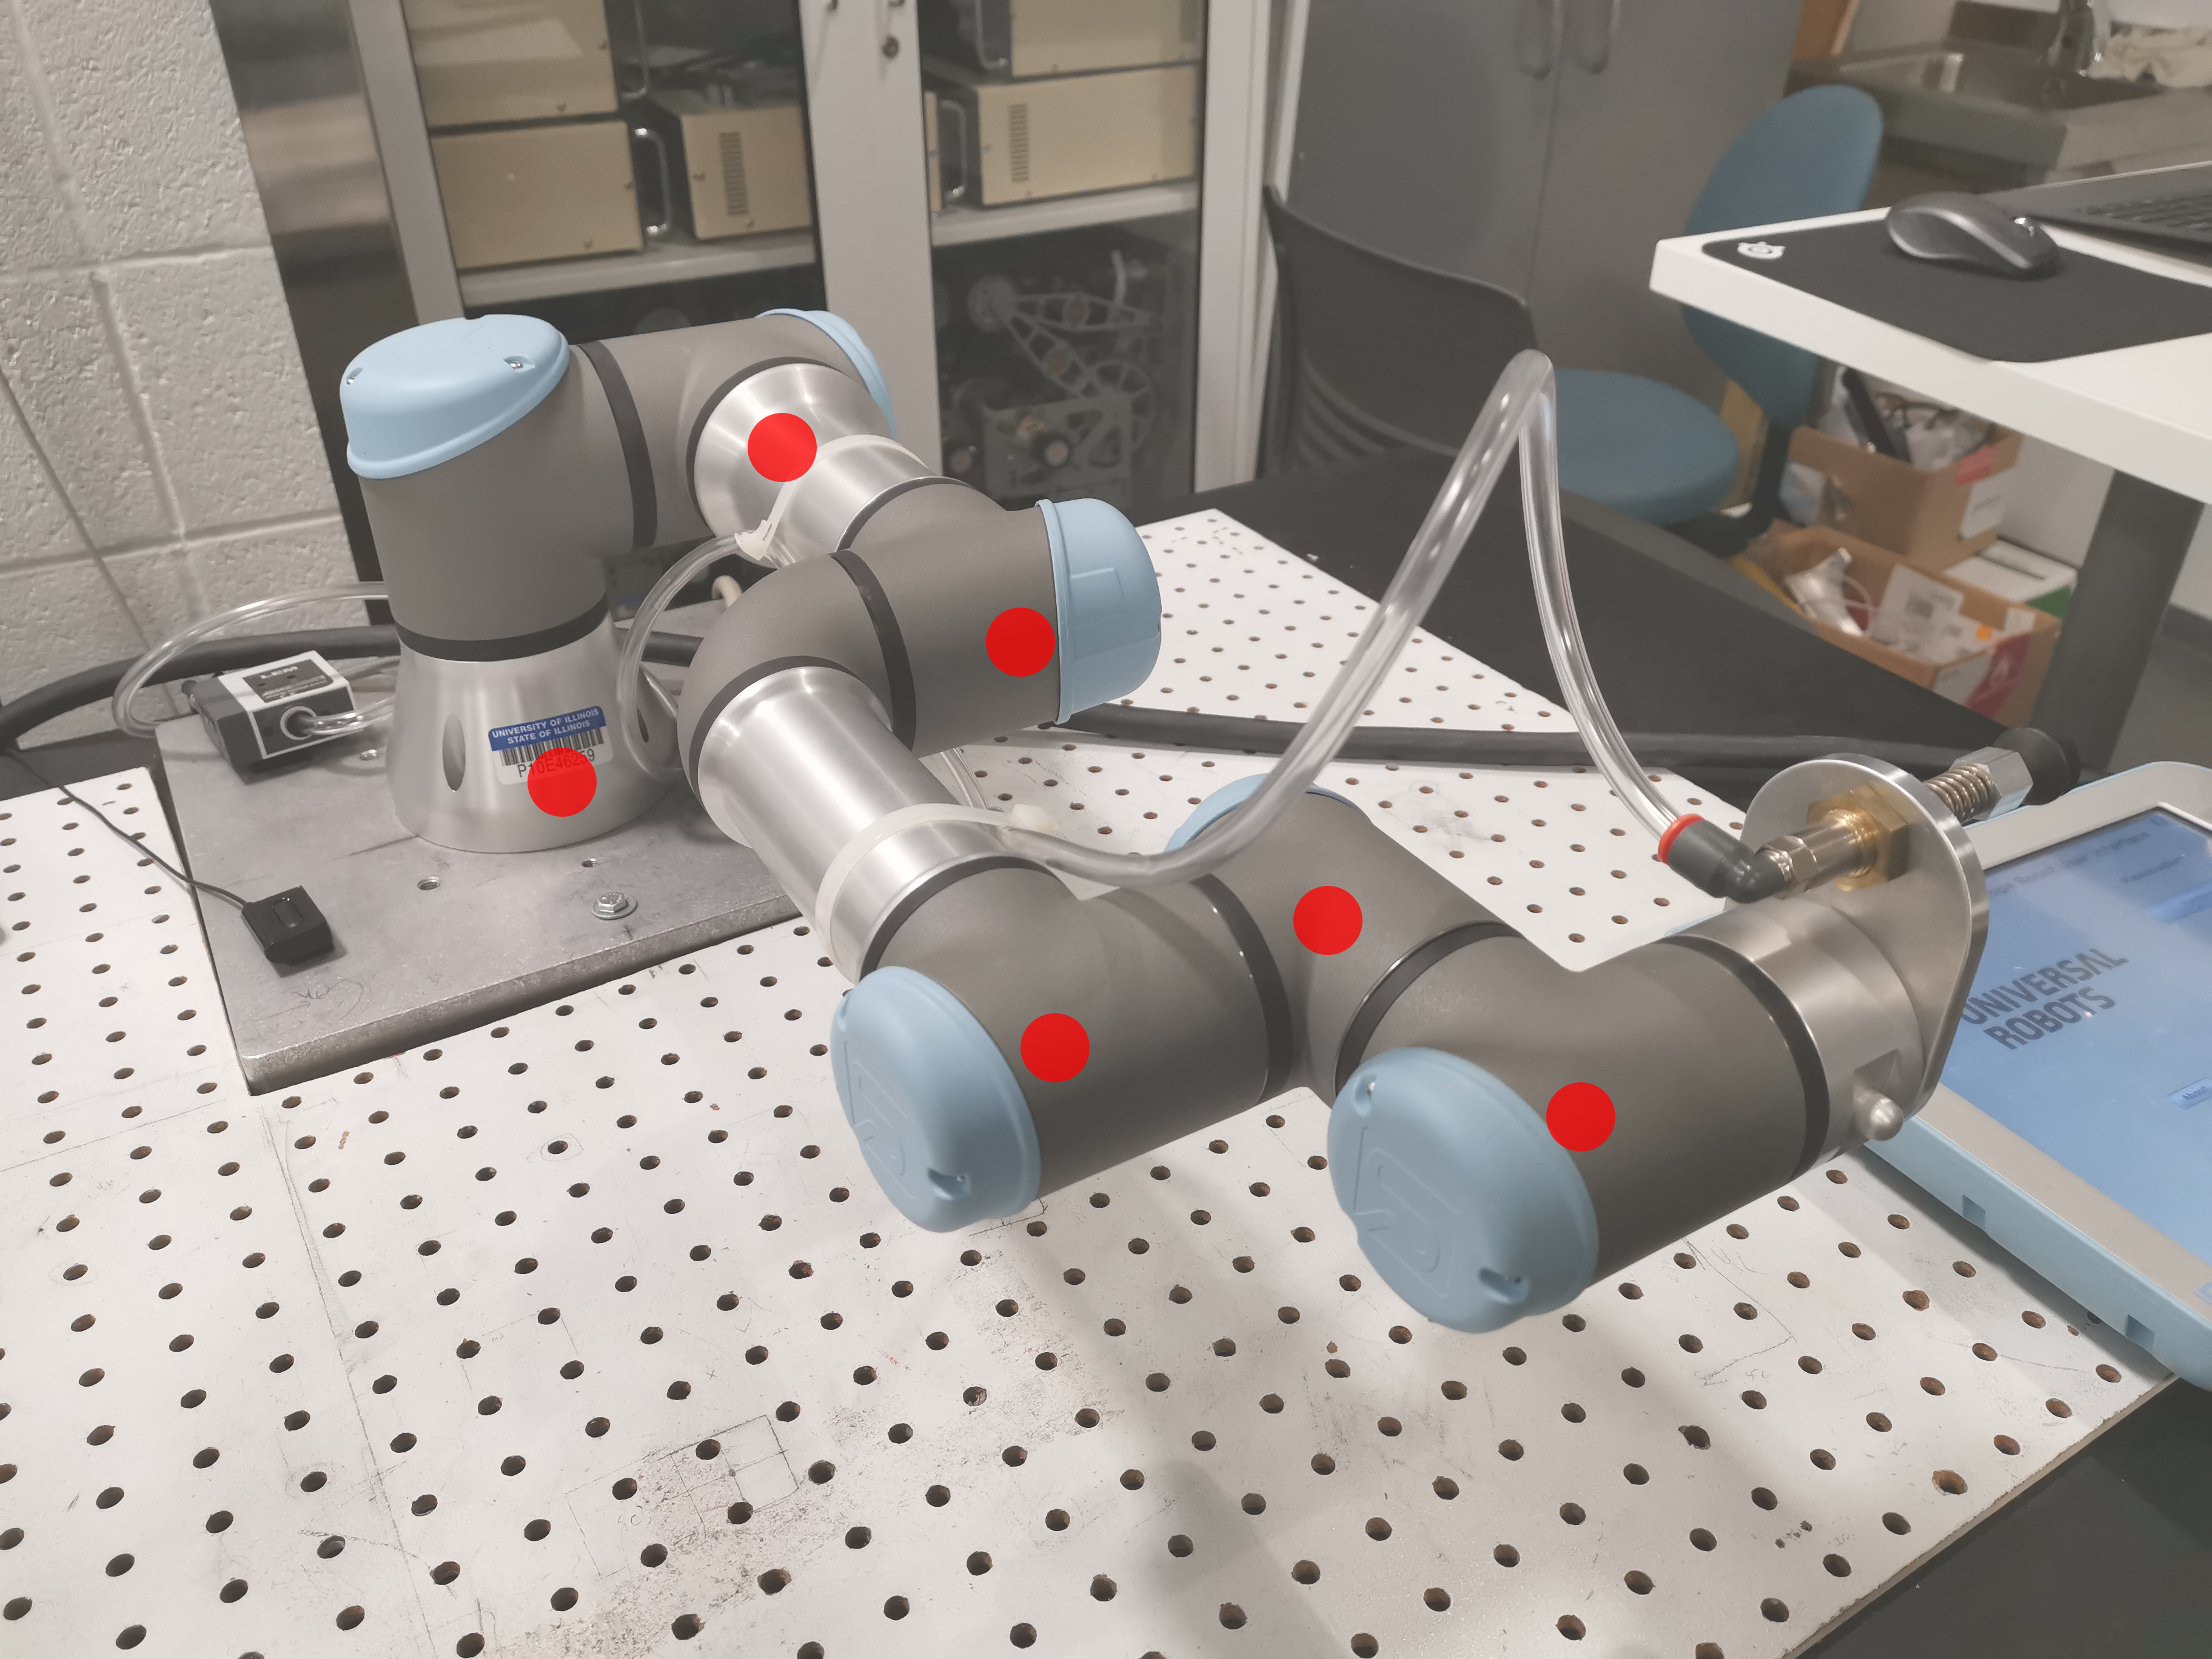
\includegraphics[height=3.4in]{image/lab4_ur3_forwardkin.jpg}
	\caption{\figlbl{UR3JC} Joint center locations on UR3e.}
\end{figure}

\begin{figure}[t]
	\centering
		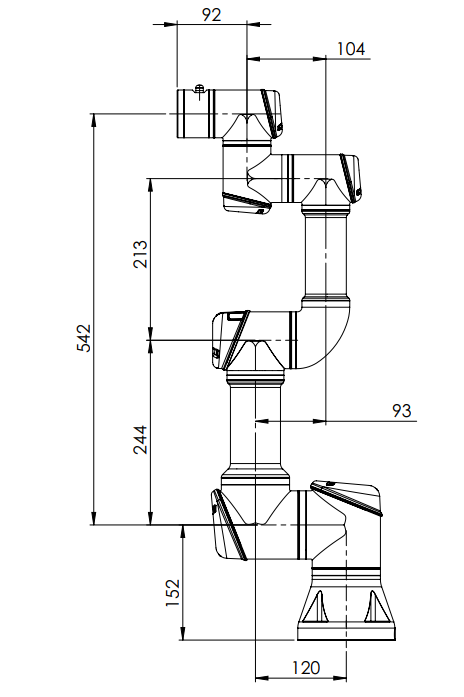
\includegraphics[height=6in]{image/lab4_ur3e_config.png}
	\caption{\figlbl{UR3Dim} Approximate Dimensions of the UR3e in mm. *EACH UR3e IS SLIGHTLY DIFFERENT DUE TO ITS MANUFACTURE TOLERANCE.}
\end{figure}


\begin{figure}[t]
	\centering
		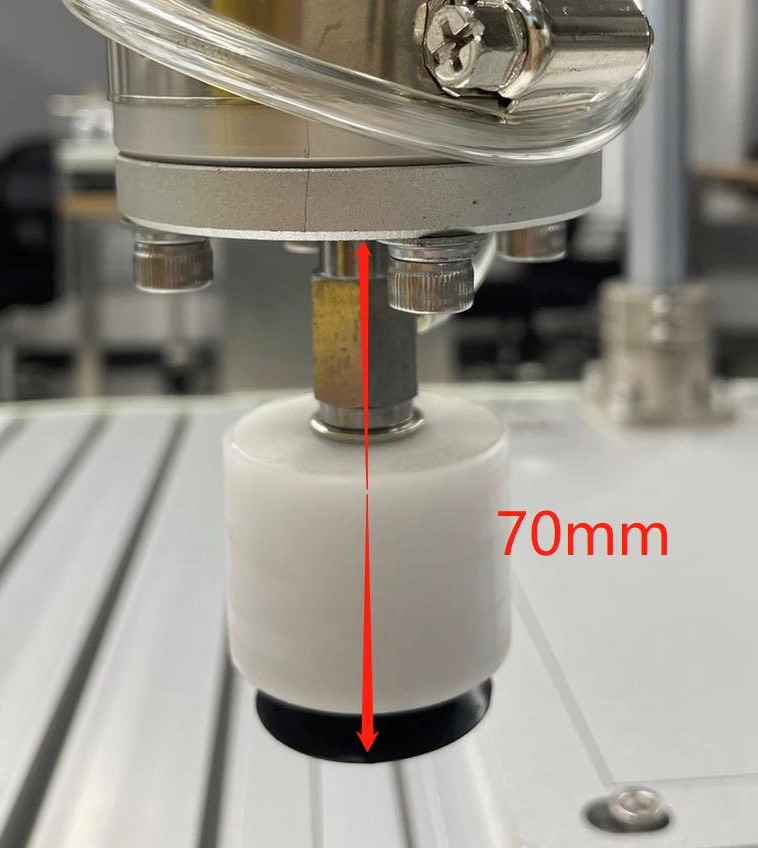
\includegraphics[height=3.5in]{image/lab4_ee_dim.jpg}
	\caption{\figlbl{EEoffset} Approximate Dimensions of the attached end effector plate and suction gripper in mm.}
\end{figure}
